\documentclass{article}
\usepackage{graphicx} % Required for inserting images
\usepackage{pgfplots}

\pgfplotsset{compat=1.18}
\usepackage[margin=0.8in]{geometry}
\usepackage{hyperref} % embedded links

%
\usepackage{amsmath}
\usepackage{amssymb }
\usepackage{amsthm}
\usepackage{nicematrix}
\usepackage{graphicx} % Required for inserting images

% More fancy stuff:
\usepackage{fancyhdr}
\pagestyle{fancy}

\fancyhead{}
\fancyfoot{}

\lhead{}
\chead{Source for TikZ for MTH 142 Comerford}
\rhead{}

\lfoot{}
\cfoot{\large{\thepage}}
\rfoot{}

\renewcommand{\footrulewidth}{1pt}

% Link formatting:
\hypersetup{
	colorlinks=true,    % false: boxed links; true: colored links
	linkcolor=blue,     % color of internal links
	citecolor=green,    % color of links to bibliography
	filecolor=magenta,  % color of file links
	urlcolor=blue       % color of external links
}

% Extra math fonts and packages:
\usepackage{mathrsfs}
\usepackage{amsfonts} 
\usepackage{amsmath}
\usepackage{mathtools}
\usepackage{amssymb}
\usepackage{amsthm}

% \newtheorem{claim}{Claim}
\newtheorem*{claim*}{Claim}


\setlength{\parindent}{0pt}

% For augmented matrices:
\newenvironment{amatrix}[1]{%
  \left[\begin{array}{*{#1}{c}|c}%
}{%
  \end{array}\right]%
}

% Source - https://tex.stackexchange.com/a/104099
% Posted by Sigur, modified by community. See post 'Timeline' for change history
% Retrieved 2026-02-17, License - CC BY-SA 3.0


% Centers the vec symbol over numbers better (\upvec 0):
\newcommand\upvec[1]{\!\vec{\,\mathrm{#1}}}

% Initiates theorem commands
\newtheorem{theorem}{Theorem}
\title{MTH 481 Optimization HW II Search Methods, FONC, SONC}
\author{T}
\date{February 17th 2026}


\begin{document}

\maketitle



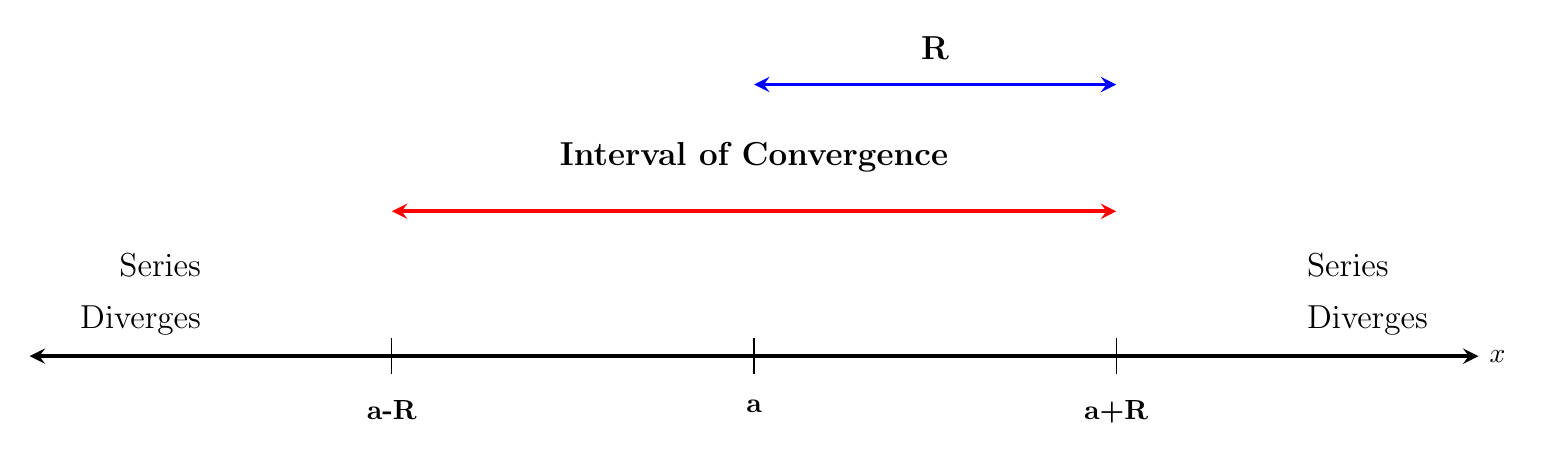
\begin{tikzpicture}[>=stealth, scale=2.3]

% Number line
\draw[<->, line width=0.5mm ] (-4,0) -- (4,0) node[right] {$x$};

% Points
\draw (-2,0.1) -- (-2,-0.1) node[below=6pt] {$\textbf{{a-R}}$};
\draw (0,0.1) -- (0,-0.1) node[below=6pt] {$\textbf{{a}}$};
\draw (2,0.1) -- (2,-0.1) node[below=6pt] {$\textbf{{a+R}}$};

% Interval of convergence arrow
\draw[<->, line width=0.5mm, red ] (-2,0.8) -- (2,0.8);


\draw[<->, line width=0.5mm, blue ] (0,1.5) -- (2,1.5);

\node at (0,1.1) {$\large \textbf{Interval of Convergence}$};
\node at (1,1.7) {$\large \textbf{R}$};

% Diverges labels
\node[left] at (-3,0.5) {$\large\text{Series}  $};
\node[left] at (-3,0.2) {$\large\text{Diverges}  $};

\node[right] at (3,0.5) {$\large\text{Series}  $};
\node[right] at (3,0.2) {$\large\text{Diverges}  $};

\end{tikzpicture}

\begin{tikzpicture}[scale=1.2]

% axes
\draw[->] (-0.5,0) -- (4,0);
\draw[->] (0,-1) -- (0,3);

% horizontal line (blue)
\draw[blue, thick] (0.1,2) -- (4,2);

% smooth curve (red)
\draw[red, thick]
    (1,1.1) .. controls (1.5,1.6) and (1.8,1.9) ..
    (2,2) ..
    controls (2.3,2.3) and (2.8,2.6) ..
    (3.6,2.9);

% intersection point
\fill[black] (2,2) circle (2.5pt);

% labels
\node[left] at (0,2) {$f(a)$};
\node[below] at (2,0) {$a$};
\node[right] at (3.6,2.9) {$s(x)$};

\end{tikzpicture}


\begin{tikzpicture}[scale=2]

% axes
\draw[->] (-0.5,0) -- (4,0);
\draw[->] (0,-0.5) -- (0,3);

% function f(x)
\draw[blue,thick]
    (0.8,1.2) .. controls (1.5,1.3) and (1.8,1.8) ..
    (2,2) ..
    controls (2.3,2.4) and (2.7,2.9) ..
    (3.2,3.2);

% tangent line at x = a
\draw[red, thick]
    (0,0) -- (3.6,3.6);

% point of tangency
\fill (2,2) circle (2.5pt);

% tick at x = a
\draw (2,0.1) -- (2,-0.1);

% labels
\node[left] at (0,2) {$f(a)$};
\node[below] at (2,0) {$a$};

\node[right] at (3.2,3.2) {$f(x)$};
\node[above right] at (2.4,2.6) {$\quad \quad \quad P_1(x)=f(a)+f'(a)(x-a)$};

\end{tikzpicture}


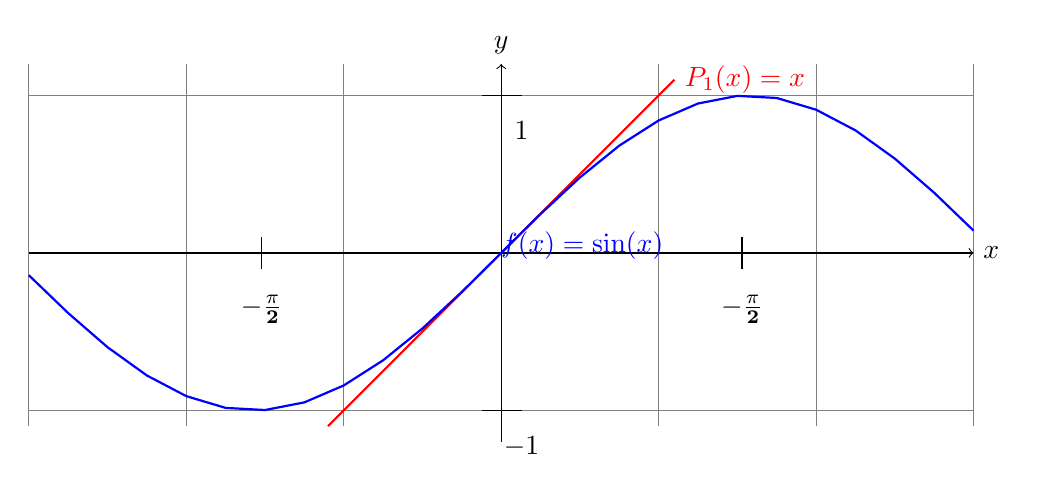
\begin{tikzpicture}[scale=2.0]% Set default domain
    % Draw grid and axes
    \draw[very thin,color=gray] (-0.1,-1.1) grid (3,1.2);
    \draw[very thin,color=gray] (-0.1,-1.1) grid (-3,1.2);
    \draw[->] (-3,0) -- (3,0) node[right] {$x$};
    \draw[->] (0,-1.2) -- (0,1.2) node[above] {$y$};

    % Plot f(x) = x
    \draw[color=red, thick, domain=-1.1:1.1] plot (\x,\x) node[right] {$P_1(x)=x$};

    % Plot f(x) = sin(x) (note the 'r' for radians)
    \draw[color=blue, thick, domain=-3:3] plot (\x, {sin(\x r)}); node[left] {\textcolor{blue}{$ \text{ } \quad  f(x)=\sin(x)$}};
    
    \draw (-2.55,0.1) -- (-2.55,-0.1) 
node[below=6pt] {$-\mathbf{\frac{\pi}{2}}$};

    \draw (0.5,0.1) -- (0.5,-0.1) 
node[below=6pt] {$-\mathbf{\frac{\pi}{2}}$};


    \draw (-1.15,1.0) -- (-0.90,1.0) 
node[below=6pt] {$1$};

    \draw (-1.15,-1.0) -- (-0.90,-1.0) 
node[below=6pt] {$-1$};

\end{tikzpicture}


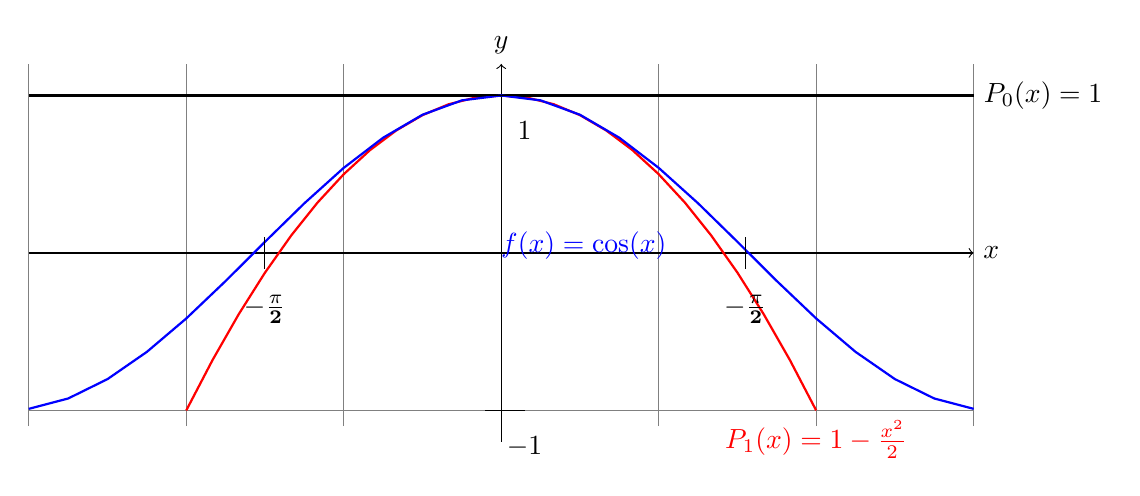
\begin{tikzpicture}[scale=2.0]% Set default domain
    % Draw grid and axes
    \draw[very thin,color=gray] (-0.1,-1.1) grid (3,1.2);
    \draw[very thin,color=gray] (-0.1,-1.1) grid (-3,1.2);
    \draw[->] (-3,0) -- (3,0) node[right] {$x$};
    \draw[->] (0,-1.2) -- (0,1.2) node[above] {$y$};

    % Plot f(x) = x
    \draw[color=red, thick, domain=-2:2] plot (\x,1-0.5*\x*\x) node[below] {$P_1(x)=1-\frac{x^2}{2}$};

    \draw[thick, domain=-3:3] plot (\x,1) node[right] {$P_0(x)=1$};

    % Plot f(x) = sin(x) (note the 'r' for radians)
    \draw[color=blue, thick, domain=-3:3] plot (\x, {cos(\x r)}); node[left] {\textcolor{blue}{$f(x)=\cos(x)$}};
    
    \draw (-2.55,0.1) -- (-2.55,-0.1) 
node[below=6pt] {$-\mathbf{\frac{\pi}{2}}$};

    \draw (0.5,0.1) -- (0.5,-0.1) 
node[below=6pt] {$-\mathbf{\frac{\pi}{2}}$};


    \draw (-1.15,1.0) -- (-0.90,1.0) 
node[below=6pt] {$1$};

    \draw (-1.15,-1.0) -- (-0.90,-1.0) 
node[below=6pt] {$-1$};

\end{tikzpicture}

\begin{tikzpicture}[>=stealth, scale=2.3]

% Number line
\draw[<->, line width=0.5mm ] (-4,0) -- (4,0) node[right] {$x$};

% Points
\draw (-1,0.1) -- (-1,-0.1) node[below=6pt] {$\textcolor{red}{\textbf{{P}}}$};
\draw (0,0.1) -- (0,-0.1) node[below=6pt] {$\textcolor{red}{\textbf{{Q}}}$};
\draw (2,0.1) -- (2,-0.1) node[below=6pt] {$\textcolor{red}{\textbf{{-Q}}}$};

\draw[<->, line width=0.5mm, red ] (-1,0.7) -- (0,0.7);

\draw[<->, line width=0.5mm, blue ] (0,0.5) -- (2,0.5);

\node at (1,0.8) {$\large \textbf{r}$};
\node at (-0.5,0.9) {$\large \textbf{R}$};

% Diverges labels




\end{tikzpicture}


\begin{tikzpicture}[scale=2.0]% Set default domain
    % Draw grid and axes
    \draw[very thin,color=gray] (-0.1,-1.1) grid (3,1.2);
    \draw[very thin,color=gray] (-0.1,-1.1) grid (-3,1.2);
    \draw[->] (-3,0) -- (3,0) node[right] {$x$};
    \draw[->] (0,-1.2) -- (0,1.2) node[above] {$y$};

    % Plot f(x) = x
    \draw[color=red, thick, domain=-3:-2] plot (\x,0);
    \draw[color=red, thick, domain=-2:-1] plot (\x,1);
    \draw[color=red, thick, domain=-1:0] plot (\x,0);
    \draw[color=red, thick, domain=0:1] plot (\x,1);
    \draw[color=red, thick, domain=1:2] plot (\x,0);
    \draw[color=red, thick, domain=2:3] plot (\x,1);

    
    \draw (1,0.1) -- (1,-0.1) 
node[below=6pt] {$1$};

    \draw (2,0.1) -- (2,-0.1) 
node[below=6pt] {$2$};

    \draw (3,0.1) -- (3,-0.1) 
node[below=6pt] {$3$};

    \draw (-1,0.1) -- (-1,-0.1) 
node[below=6pt] {$-1$};

    \draw (-2,0.1) -- (-2,-0.1) 
node[below=6pt] {$-2$};

    \draw (-3,0.1) -- (-3,-0.1) 
node[below=6pt] {$-3$};

\end{tikzpicture}

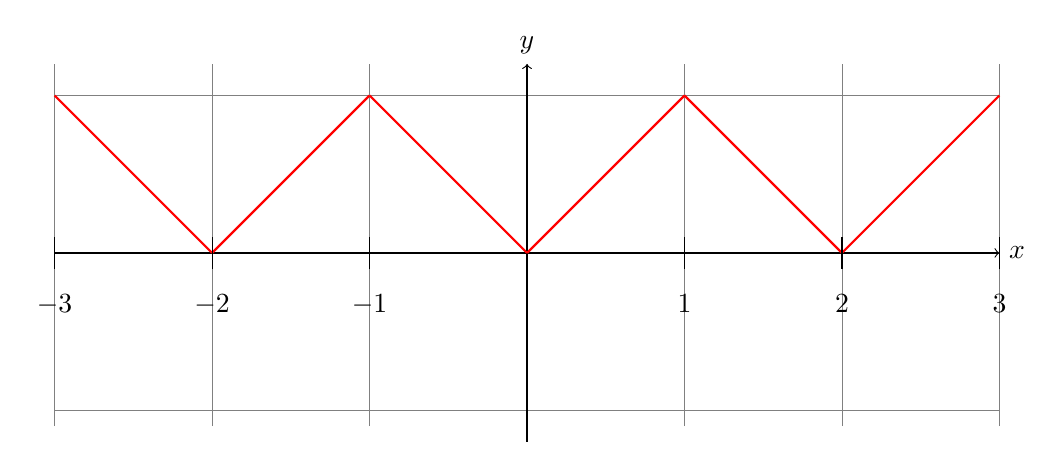
\begin{tikzpicture}[scale=2.0]% Set default domain
    % Draw grid and axes
    \draw[very thin,color=gray] (-0.1,-1.1) grid (3,1.2);
    \draw[very thin,color=gray] (-0.1,-1.1) grid (-3,1.2);
    \draw[->] (-3,0) -- (3,0) node[right] {$x$};
    \draw[->] (0,-1.2) -- (0,1.2) node[above] {$y$};

    % Plot f(x) = x
    \draw[color=red, thick, domain=-3:-2] plot (\x,-\x-2);
    \draw[color=red, thick, domain=-2:-1] plot (\x,\x+2);
    \draw[color=red, thick, domain=-1:0] plot (\x,-\x);
    \draw[color=red, thick, domain=0:1] plot (\x,\x);
    \draw[color=red, thick, domain=1:2] plot (\x,-\x+2);
    \draw[color=red, thick, domain=2:3] plot (\x,\x-2);

    
    \draw (1,0.1) -- (1,-0.1) 
node[below=6pt] {$1$};

    \draw (2,0.1) -- (2,-0.1) 
node[below=6pt] {$2$};

    \draw (3,0.1) -- (3,-0.1) 
node[below=6pt] {$3$};

    \draw (-1,0.1) -- (-1,-0.1) 
node[below=6pt] {$-1$};

    \draw (-2,0.1) -- (-2,-0.1) 
node[below=6pt] {$-2$};

    \draw (-3,0.1) -- (-3,-0.1) 
node[below=6pt] {$-3$};

\end{tikzpicture}

\begin{tikzpicture}[scale=2.0]% Set default domain
    % Draw grid and axes
    \draw[very thin,color=gray] (-0.1,-1.1) grid (1.5,1.2);
    \draw[very thin,color=gray] (-0.1,-1.1) grid (-1.5,1.2);
    \draw[->] (-1.3,0) -- (1.6,0) node[right] {$x$};
    \draw[->] (0,-1.2) -- (0,1.2) node[above] {$y$};

    % Plot f(x) = x
    
    \draw[color=red, thick, domain=-1:0] plot (\x,0);
    \draw[color=red, thick, domain=0:1] plot (\x,1);

    \draw[color=red, thick, domain=-1.5:-1] plot (\x,1);
    \draw[color=red, thick, domain=1:1.5] plot (\x,0);

    \draw (1,0.1) -- (1,-0.1) 
node[below=6pt] {$\pi$};

    \draw (-1,0.1) -- (-1,-0.1) 
node[below=6pt] {$-\pi$};


    \filldraw[fill=white] (-1,1) circle (1pt);
    \filldraw[fill=red] (-1,0) circle (1pt);
    \filldraw[fill=white] (1,1) circle (1pt);
    \filldraw[fill=red] (1,0) circle (1pt);
    \filldraw[fill=white] (0,0) circle (1pt);
    \filldraw[fill=red] (0,1) circle (1pt);
    


    

\end{tikzpicture}

 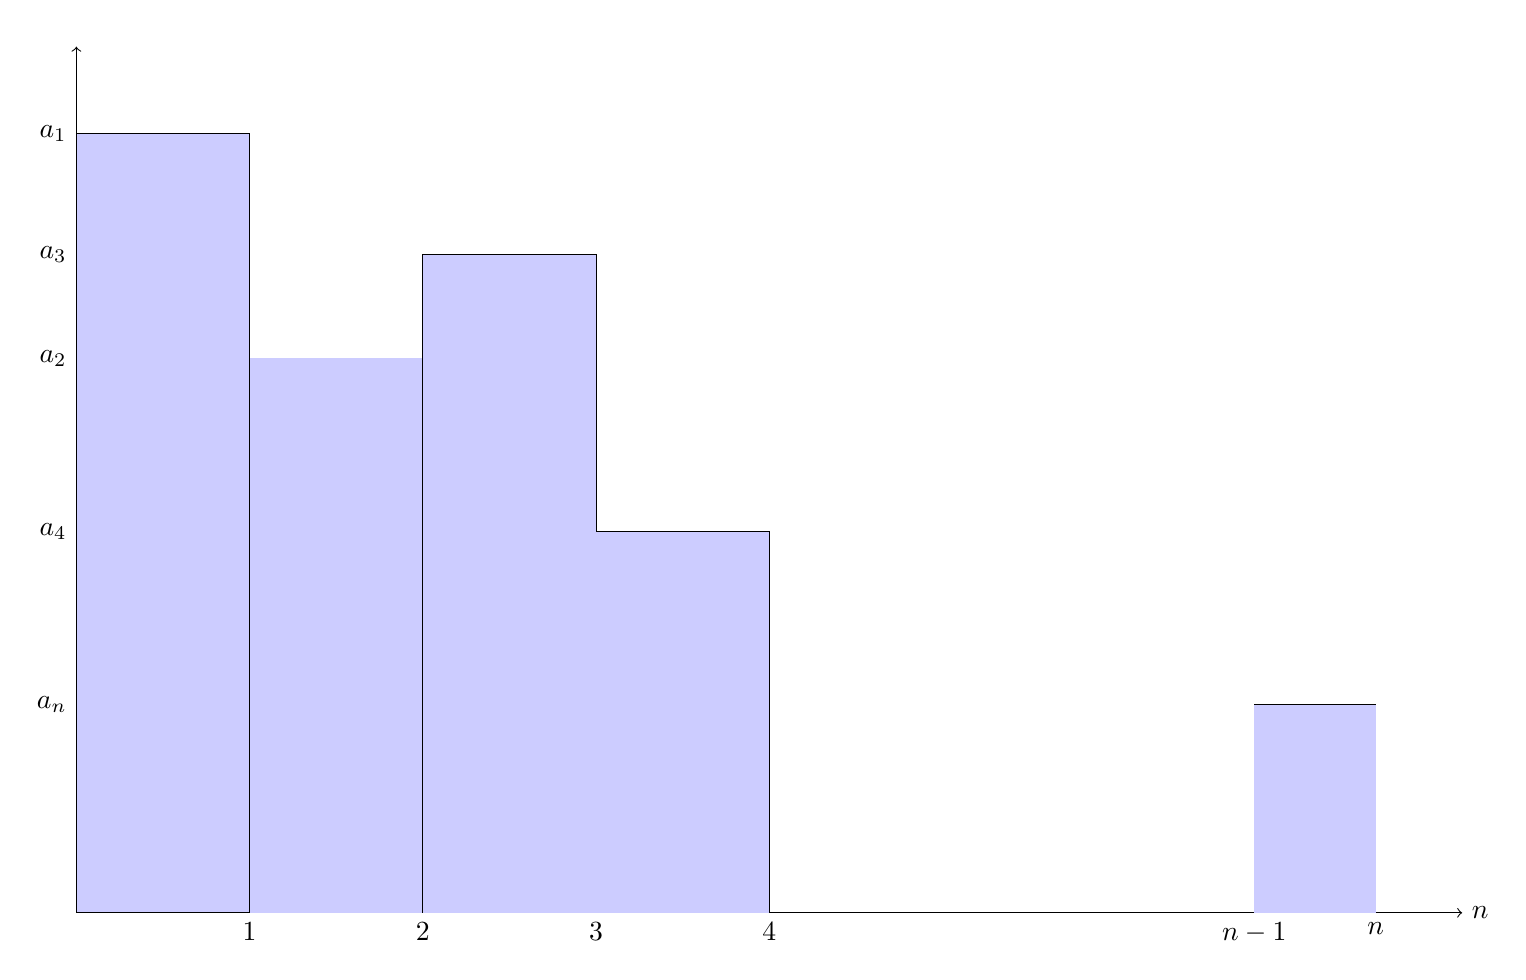
\begin{tikzpicture}[scale=2.2]

    % Axes
    \draw[->] (0,0) -- (8,0) node[right] {$n$};
    \draw[->] (0,0) -- (0,5) node[above] {};

    % Y-axis labels
    \node[left] at (0,4.5) {$a_1$};
    \node[left] at (0,3.8) {$a_3$};
    \node[left] at (0,3.2) {$a_2$};
    \node[left] at (0,2.2) {$a_4$};
    \node[left] at (0,1.2) {$a_n$};

    % X-axis ticks
    \foreach \x in {1,2,3,4}
        \draw (\x,0) -- (\x,0.0) node[below] {\x};

    \draw (6.8,0) -- (6.8,0.0) node[below] {$n-1$};
    \draw (7.5,0) -- (7.5,0.0) node[below] {$n$};

    % Rectangles (example heights to match sketch)
    \fill[blue!20] (0,0) rectangle (1,4.5);   % a1
    \draw (0,0) rectangle (1,4.5);   % a1
    \draw (1,0) rectangle (2,3.2);   % a2
    \fill[blue!20]  (1,0) rectangle (2,3.2);   % a2

    \draw (2,0) rectangle (3,3.8);   % a3
    \fill[blue!20]  (2,0) rectangle (3,3.8);   % a3
    \draw (3,0) rectangle (4,2.2);   % a4
    \fill[blue!20]  (3,0) rectangle (4,2.2);   % a4
    \draw (6.8,0) rectangle (7.5,1.2); % a_n
    \fill[blue!20]  (6.8,0) rectangle (7.5,1.2); % a_n

    \end{tikzpicture}

         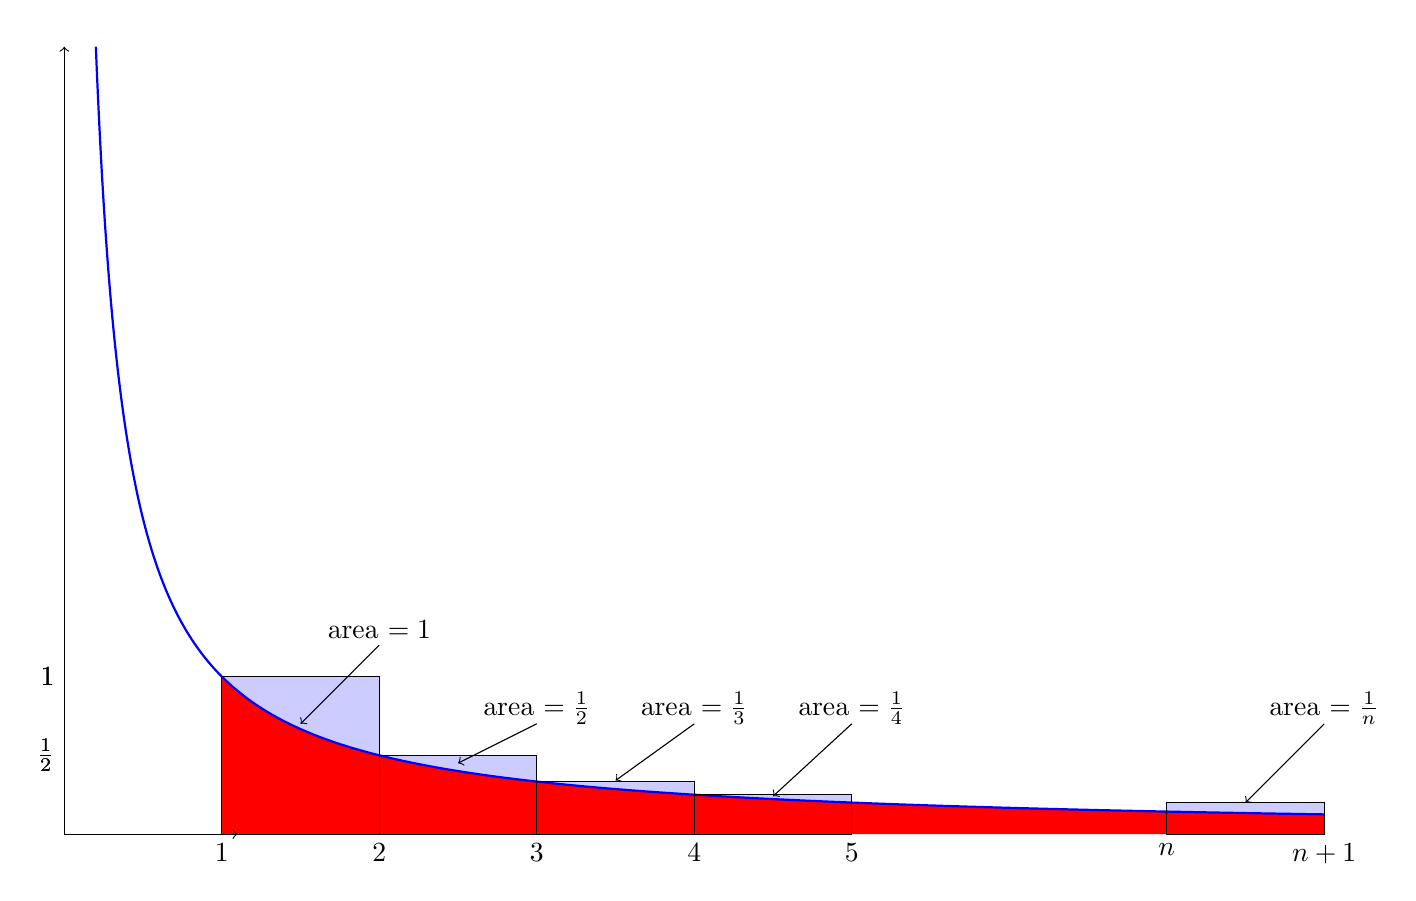
\begin{tikzpicture}[scale=2]

      % Axes

      % Rectangles (example heights to match sketch)
      \fill[blue!20] (1,0) rectangle (2,1);   % a1
      \fill[blue!20] (2,0) rectangle (3,0.5);   % a1
      \fill[blue!20] (3,0) rectangle (4,1/3);   % a1
      \fill[blue!20] (4,0) rectangle (5,1/4);   % a1
      \fill[blue!20] (4,0) rectangle (5,1/4);   % a1
      \fill[blue!20] (7,0) rectangle (8,1/5);   % a1


      \fill[red, domain=1:8, samples=200]
          (1,0)
          -- plot (\x, {1/\x})
          -- (8,0)
          -- cycle;

      % Draw the curve on top
      \draw[blue, thick, domain=1:8, samples=200]
          plot (\x, {1/\x});

      % Draw the curve on top
      \draw[blue, thick, domain=0.2:1, samples=200]
          plot (\x, {1/\x});

      \draw (1,0) rectangle (2,1);   % a1
      \draw (2,0) rectangle (3,1/2);   % a1
      \draw (3,0) rectangle (4,1/3);   % a1
      \draw (4,0) rectangle (5,1/4);   % a1
      \draw (4,0) rectangle (5,1/4);   % a1
      \draw (7,0) rectangle (8,1/5);   % a1

      \draw[->] (0,0) -- (1.1,0) node[right] {};
      \draw[->] (0,0) -- (0,5) node[above] {};

      % Y-axis labels
      \node[left] at (0,1) {$1$};
      \node[left] at (0,0.5) {$\frac{1}{2}$};
      \node[left] at (0,1) {$1$};
      \node[left] at (0,0.5) {$\frac{1}{2}$};

      % X-axis ticks
      \foreach \x in {1,2,3,4,5}
          \draw (\x,0) -- (\x,0.0) node[below] {\x};

      \draw (7,0) -- (7,0.0) node[below] {$n$};
      \draw (8,0) -- (8,0.0) node[below] {$n+1$};

      %node area info
      \node at (2,1.3) {area $=1$};
      \draw[->] (2,1.2) -- (1.5,.7);

      \node at (3,0.8) {area $=\frac{1}{2}$};
      \draw[->] (3,0.70) -- (2.5,0.45);

      \node at (4,0.8) {area $=\frac{1}{3}$};
      \draw[->] (4,0.70) -- (3.5,0.34);

      \node at (5,0.8) {area $=\frac{1}{4}$};
      \draw[->] (5,0.70) -- (4.5,0.24);

      \node at (8,0.8) {area $=\frac{1}{n}$};
      \draw[->] (8,0.70) -- (7.5,0.20);

      \end{tikzpicture}

         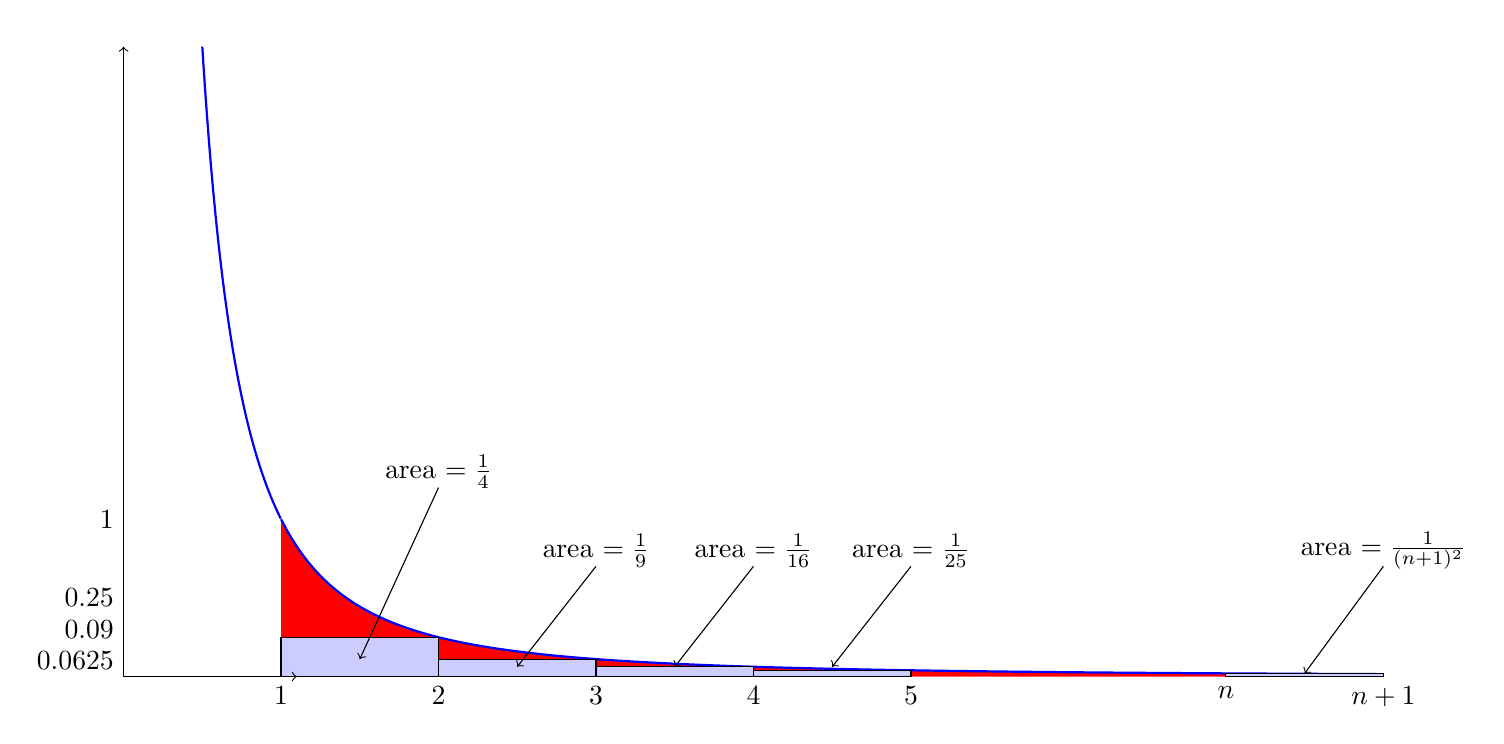
\begin{tikzpicture}[scale=2]

    % Axes



    \fill[red, domain=1:8, samples=200]
        (1,0)
        -- plot (\x, {1/(\x *\x)})
        -- (8,0)
        -- cycle;

    % Draw the curve on top
    \draw[blue, thick, domain=0.5:1, samples=200]
        plot (\x, {1/(\x * \x)});

    % Draw the curve on top
    \draw[blue, thick, domain=1:8, samples=200]
        plot (\x, {1/(\x * \x)});

    % Rectangles (example heights to match sketch)
    \fill[blue!20] (1,0) rectangle (2,1/4);   % a1
    \fill[blue!20] (2,0) rectangle (3,1/9);   % a1
    \fill[blue!20] (3,0) rectangle (4,1/16);   % a1
    \fill[blue!20] (4,0) rectangle (5,1/25);   % a1
    \fill[blue!20] (7,0) rectangle (8,1/50);   % a1

    \draw (1,0) rectangle (2,1/4);   % a1
    \draw (2,0) rectangle (3,1/9);   % a1
    \draw (3,0) rectangle (4,1/16);   % a1
    \draw (4,0) rectangle (5,1/25);   % a1
    \draw (7,0) rectangle (8,1/50);   % a1

    \draw[->] (0,0) -- (1.1,0) node[right] {};
    \draw[->] (0,0) -- (0,4) node[above] {};

    % Y-axis labels
    \node[left] at (0,1) {$1$};
    \node[left] at (0,0.5) {0.25};
    \node[left] at (0,0.3) {0.09};
    \node[left] at (0,0.1) {0.0625};


    % X-axis ticks
    \foreach \x in {1,2,3,4,5}
        \draw (\x,0) -- (\x,0.0) node[below] {\x};

    \draw (7,0) -- (7,0.0) node[below] {$n$};
    \draw (8,0) -- (8,0.0) node[below] {$n+1$};

    %node area info
    \node at (2,1.3) {area $=\frac{1}{4}$};
    \draw[->] (2,1.2) -- (1.5,1/9);

    \node at (3,0.8) {area $=\frac{1}{9}$};
    \draw[->] (3,0.70) -- (2.5,1/16);

    \node at (4,0.8) {area $=\frac{1}{16}$};
    \draw[->] (4,0.70) -- (3.5,1/16);

    \node at (5,0.8) {area $=\frac{1}{25}$};
    \draw[->] (5,0.70) -- (4.5,1/16);

    \node at (8,0.8) {area $=\frac{1}{(n+1)^2}$};
    \draw[->] (8,0.70) -- (7.5,1/49);

    \end{tikzpicture}

      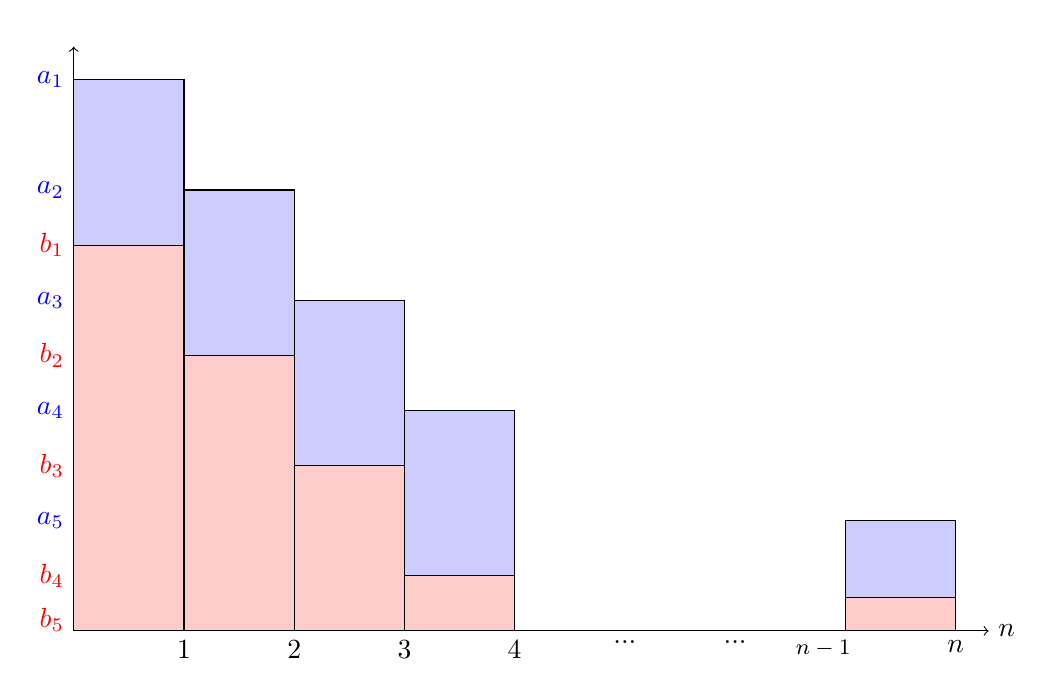
\begin{tikzpicture}[scale=1.4]

      % Axes
      \draw[->] (0,0) -- (8.3,0) node[right] {$n$};
      \draw[->] (0,0) -- (0,5.3) node[above] {};

      % Y-axis labels
      \node[left] at (0,5) {\textcolor{blue}{$a_1$}};
      \node[left] at (0,4) {\textcolor{blue}{$a_2$}};
      \node[left] at (0,3) {\textcolor{blue}{$a_3$}};
      \node[left] at (0,2) {\textcolor{blue}{$a_4$}};
      \node[left] at (0,1) {\textcolor{blue}{$a_5$}};

      \node[left] at (0,3.5) {\textcolor{red}{$b_1$}};
      \node[left] at (0,2.5){\textcolor{red}{$b_2$}};
      \node[left] at (0,1.5) {\textcolor{red}{$b_3$}};
      \node[left] at (0,0.5) {\textcolor{red}{$b_4$}};

      \node[left] at (0,0.1) {\textcolor{red}{$b_5$}};

      % X-axis ticks
      \foreach \x in {1,2,3,4}
          \draw (\x,0) -- (\x,0.0) node[below] {\x};

      \draw (5,0) -- (6,0.0) node[below] {...};
      \draw (4,0) -- (5,0.0) node[below] {...};
      

      \draw (6.8,0) -- (6.8,0.0) node[below] {\footnotesize $n-1$};
      \draw (8,0) -- (8,0.0) node[below] {$n$};

      % Rectangles (example heights to match sketch)
      \fill[blue!20] (0,0) rectangle (1,5);   % a1
      \draw (0,0) rectangle (1,5);   % a1
      
      \fill[blue!20] (1,0) rectangle (2,4);   % a1
      \draw (1,0) rectangle (2,4);   % a1

      \fill[blue!20] (2,0) rectangle (3,3);   % a1
      \draw (2,0) rectangle (3,3);   % a1

      \fill[blue!20] (3,0) rectangle (4,2);   % a1
      \draw (3,0) rectangle (4,2);   % a1

      \fill[blue!20] (7,0) rectangle (8,1);   % a1
      \draw (7,0) rectangle (8,1);   % a1

      % Rectangles (example heights to match sketch)
      \fill[red!20] (0,0) rectangle (1,3.5);   % a1
      \draw (0,0) rectangle (1,3.5);   % a1
      
      \fill[red!20] (1,0) rectangle (2,2.5);   % a1
      \draw (1,0) rectangle (2,2.5);   % a1

      \fill[red!20] (2,0) rectangle (3,1.5);   % a1
      \draw (2,0) rectangle (3,1.5);   % a1

      \fill[red!20] (3,0) rectangle (4,0.5);   % a1
      \draw (3,0) rectangle (4,0.5);   % a1

      \fill[red!20] (7,0) rectangle (8,0.3);   % a1
      \draw (7,0) rectangle (8,0.3);   % a1


      \end{tikzpicture}

      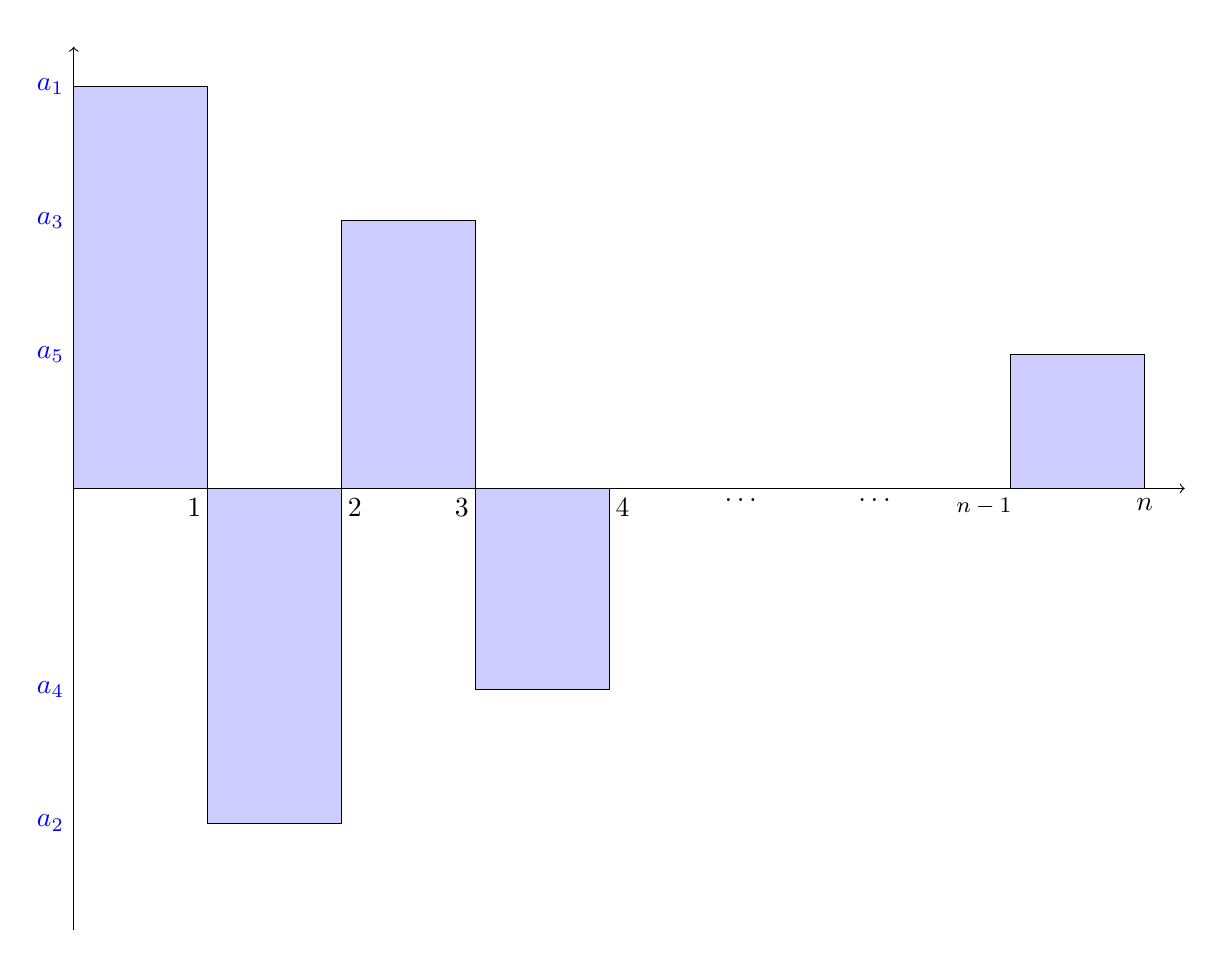
\begin{tikzpicture}[scale=1.7]

    % Axes
    \draw[->] (0,0) -- (8.3,0) node[right] {};
    \draw[->] (0,-3.3) -- (0,3.3) node[above] {};

    % Y-axis labels
    \node[left] at (0,3) {\textcolor{blue}{$a_1$}};
    \node[left] at (0,-2.5) {\textcolor{blue}{$a_2$}};
    \node[left] at (0,2) {\textcolor{blue}{$a_3$}};
    \node[left] at (0,-1.5) {\textcolor{blue}{$a_4$}};
    \node[left] at (0,1) {\textcolor{blue}{$a_5$}};



    % Rectangles (example heights to match sketch)
    \fill[blue!20] (0,0) rectangle (1,3);   % a1
    \draw (0,0) rectangle (1,3);   % a1
    
    \fill[blue!20] (1,0) rectangle (2,-2.5);   % a1
    \draw (1,0) rectangle (2,-2.5);   % a1

    \fill[blue!20] (2,0) rectangle (3,2);   % a1
    \draw (2,0) rectangle (3,2);   % a1

    \fill[blue!20] (3,0) rectangle (4,-1.5);   % a1
    \draw (3,0) rectangle (4,-1.5);   % a1

    \fill[blue!20] (7,0) rectangle (8,1);   % a1
    \draw (7,0) rectangle (8,1);   % a1

    % X-axis ticks
    \foreach \x in {1,3}
        \draw (\x-0.1,0) -- (\x-0.1,0.0) node[below] {\x};

    \foreach \x in {2,4}
        \draw (\x+0.1,0) -- (\x+0.1,0.0) node[below] {\x};

    \draw (5,0) -- (6,0.0) node[below] {$\dots$};
    \draw (4,0) -- (5,0.0) node[below] {$\dots$};
    

    \draw (6.8,0) -- (6.8,0.0) node[below] {\footnotesize $n-1$};
    \draw (8,0) -- (8,0.0) node[below] {$n$};

    \end{tikzpicture}

\begin{tikzpicture}[scale=2]

% positions
\def\y{0}
\def\xsep{1.8}

\node (S0) at (0*\xsep,\y -.1) {$0$};
\node (S2) at (1*\xsep,\y -.1) {$S_2$};
\node (S4) at (2*\xsep,\y -.1) {$S_4$};
\node (S)  at (3*\xsep,\y -.1) {$S$};
\node (S5) at (4*\xsep,\y -.1) {$S_5$};
\node (S3) at (5*\xsep,\y -.1) {$S_3$};
\node (S1) at (6*\xsep,\y -.1) {$S_1$};


% baseline
\draw (-0.5*\xsep,\y) -- (6.5*\xsep,\y);

% small ticks
\foreach \n in {S0,S2,S4,S,S5,S3,S1}
  \draw (\n) -- ++(0,0.15);

% nested arcs
\draw[->,bend left=60] (S0) to (S1);
\draw[->,bend left=50] (S2) to (S1);
\draw[->,bend left=50] (S2) to (S3);
\draw[->,bend left=50] (S4) to (S3);
\draw[->,bend left=40] (S4) to (S5);

\end{tikzpicture}

\begin{tikzpicture}[scale=2.0]% Set default domain
    % Draw grid and axes
    \draw[very thin,color=gray] (-0.1,-1.1) grid (3,1.3);
    \draw[very thin,color=gray] (-0.1,-1.1) grid (-3,1.3);
    \draw[->] (-3,0) -- (3,0) node[right] {$x$};
    \draw[->] (0,-1.2) -- (0,1.2) node[above] {$y$};


  \draw[blue, thick, domain=-1:1, samples=100]
    plot (\x, {exp(\x)});

    \draw (-1,0.1) -- (-1,-0.1) 
node[below=6pt] {$-\mathbf{\frac{\pi}{2}}$};

    \draw (1,0.1) -- (1,-0.1) 
node[below=6pt] {$-\mathbf{\frac{\pi}{2}}$};

\end{tikzpicture}

\begin{tikzpicture}[scale=2]

    % Choose the base a
    \def\a{2} % change this to any a > 0, a ≠ 1

    % Axes
    \draw[->] (-2,0) -- (3.5,0) node[right] {$x$};
    \draw[->] (0,-0.5) -- (0,4) node[above] {$y$};

    % Plot a^x
    \draw[thick, red, domain=-2:3.5] 
        plot(\x, { 0.7+(0.3)* \a^(\x)} );


    % y0 mark
    \draw[dashed] (0,1) -- (3.5,1);
    \node[above] at (0,1) {\textcolor{blue}{$y_0$}};

\end{tikzpicture}

\begin{tikzpicture}[scale=2]

    % Choose the base a
    \def\a{2} % change this to any a > 0, a ≠ 1

    % Axes
    \draw[->] (-2,0) -- (3.5,0) node[right] {$x$};
    \draw[->] (0,-0.5) -- (0,4) node[above] {$y$};

    % Plot a^x
    \draw[thick, red, domain=-2:3.5] 
        plot(\x, { 0.7+(0.3)* \a^(-1* \x)} );


    % y0 mark
    \draw[dashed] (0,1) -- (3.5,1);
    \node[above] at (0,1) {\textcolor{blue}{$y_0$}};

\end{tikzpicture}

\begin{tikzpicture}[scale=2]

    % Choose the base a
    \def\a{2} % change this to any a > 0, a ≠ 1

    % Axes
    \draw[->] (-2,0) -- (3.5,0) node[right] {$x$};
    \draw[->] (0,-0.5) -- (0,4) node[above] {$y$};

    % Plot a^x
    \draw[thick, red, domain=-2:3.5] 
        plot(\x, { 0.7+(0.3)* \a^(-1* \x)} );


    % y0 mark
    \draw[dashed] (0,1) -- (3.5,1);
    \node[above] at (0,1) {\textcolor{blue}{$y_0$}};

\end{tikzpicture}


\begin{tikzpicture}[>=stealth]

% Axes
\draw[->] (0,-2) -- (0,2) node[above] {};
\draw[->] (0,0) -- (8,0) node[right] {$t$};

% Labels for B
\node[left,red] at (0,1.5) {$B>0$};
\node[left,blue] at (0,-1.5) {$B<0$};

% Upper curve (B > 0)
\draw[thick, domain=0:7, smooth, samples=100, red]
    plot (\x, {1.5*exp(-0.4*\x)});

% Lower curve (B < 0)
\draw[thick, domain=0:7, smooth, samples=100, blue]
    plot (\x, {-1.5*exp(-0.4*\x)});

% Middle line (B = 0)
\draw[thick] (0,0) -- (7,0);

% Annotation
\node[right] at (7,0.3) {$H=20 \quad (B=0)$};

\end{tikzpicture}

\begin{tikzpicture}[scale=2]

    % Choose the base a
    \def\a{2} % change this to any a > 0, a ≠ 1

    % Axes
    \draw[->] (-2,0) -- (3.5,0) node[right] {$x$};
    \draw[->] (0,-0.5) -- (0,4) node[above] {$y$};

    % Plot a^x
    \draw[thick, red, domain=-2:3.5] 
        plot(\x, { (5)* \a^(-1* \x)} );


    % y0 mark
    \draw[dashed] (0,1) -- (3.5,1);
    \node[above] at (0,1) {\textcolor{blue}{$y_0$}};

\end{tikzpicture}

\begin{tikzpicture}
\begin{axis}[
    axis lines=middle,
    xmin=-1, xmax=4,
    ymin=0, ymax=6,
    samples=200,
    domain=-1:4,
    xlabel={$t$},
    ylabel={$s$},
    xtick={1},
    xticklabels={$1$},
    ytick={5},
    yticklabels={$5$},
    enlargelimits=true
]

% Function plot (blue)
\addplot[thick, blue] {5*exp(-(1-x)^2)};

\end{axis}
\end{tikzpicture}

%7.4.2 integral of ellipse, ellipse_a_b.png 
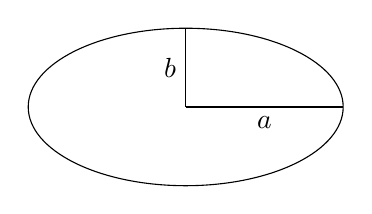
\begin{tikzpicture}
    \draw (0,0) ellipse (2cm and 1cm);

% axes
\draw[-] (0,0) -- (2,0);
\draw[-] (0,0) -- (0,1);
\node[left] at (0,0.5) {$b$};
\node[below] at (1,0) {$a$};

    
\end{tikzpicture}

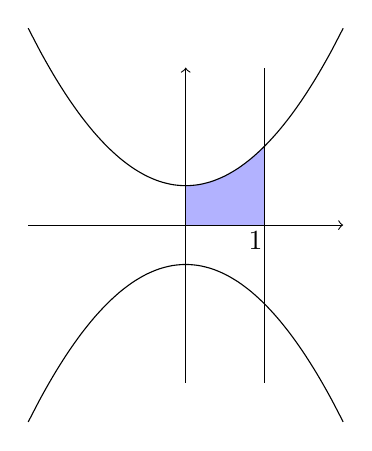
\begin{tikzpicture}

% Shaded region (top-right quadrant bounded by x=0, x=1, y=0, and upper curve)
\fill[blue!30]
    (0,0) -- (1,0)
    -- plot[domain=1:0] (\x,{0.5*\x*\x + 0.5})
    -- cycle;

% Axes
\draw[->] (-2,0) -- (2,0);
\draw[->] (0,-2) -- (0,2);

% Curves
\draw[domain=-2:2,smooth] plot (\x,{0.5*\x*\x + 0.5}); % upper curve
\draw[domain=-2:2,smooth] plot (\x,{-0.5*\x*\x - 0.5}); % lower curve

% Vertical line x=1
\draw (1,-2) -- (1,2);

% Label "1"
\node[left] at (1.1,-0.2) {1};

\end{tikzpicture}


\end{document}
